\documentclass[]{article}

\usepackage{amsmath}
\usepackage[]{graphicx}
\usepackage{subfigure}
\usepackage[latin1]{inputenc}
\usepackage{comment}
\usepackage{url}
%\usepackage{biblatex} 
%\usepackage[pdftex]{graphicx}
\usepackage{anysize}
\marginsize{3cm}{3cm}{2cm}{2.5cm}%l r t b

\title{Gaze Enhanced Speech Recognition for Hands-Free HCI}
%\title{Controlling a smart phone using gaze gestures}
%\title{Gaze gestures as an innovative HCI method for smartphone like devices}
 
\author{Matheus Portela, David Rozado}

\setlength\parindent{0pt} %no indentation in paragraphs
% Document starts
\begin{document}

\maketitle

\section{Abstract}
This is the abstract

\section{Introduction}
In computer science speech recognition refers to the computational translation of spoken words into text.

Using speech to create or edit documents and e-mail offers the potential to be a faster a more natural way to interact
with computers as well as a hands-free modality with obvious positive implications for handicapped users or
scenarios were computer users have their hands engaged in other tasks (for example surgeons in the operating room).

Although there has been a significant increase in the accuracy performance of speech recognition software, error
rates still make the technology cumbersome to use for everyday interaction  and it still requires a relatively long
learning curve to master it.

The correction of errors can be carried out manually with a traditional keyboard and mouse to select and retype the
misrecognized word. This modality can be perfectly valid for some scenarios, but this interaction modalities is not
hands-free anymore.  Correcting misrecognized with voice is an alternative that while remaining hands-free is extremely
error-prone and frustrating for users, especially when trying to correct ``difficult'' words or when being used by users
with an accent.

In this work, we propose the enhancement of speech recognition software with gaze tracking technology to speed up the
correction of misrecognized words and to make speech recognition truly hands-free.

A gaze tracking system tracks the point of regard (PoR) of the user on the screen by monitoring the users pupils while
sitting in front of a computer \cite{Rozado2012a}.

In the experimental part of his work, we compared three modalities of correcting misrecognized words during  a speech
recognition task:
\begin{itemize}
  \item usage of the traditional keyboard and mouse
  \item usage of voice
  \item usage of gaze
\end{itemize}



\section{Methodology}
Methodology introduction

\subsection{Eye Tracking}
Eyes are used by humans to obtain information about the surroundings and to
communicate information. When something attracts our attention, we position our
gaze on it, thus performing a \textit{fixation}. A fixation usually has a
duration of at least 150 milliseconds (ms). The fast eye movements that
occur between fixations are known as \textit{saccades}, and they are used to
reposition the eye so that the object of interest is projected onto the fovea.
The direction of gaze thus reflects the focus of 
\textit{attention} and also provides an indirect hint for \textit{intention}
\cite{velichkovsky}.


A video-based gaze tracking system seeks to find where a person is looking, i.e.
the Point of Regard (PoR), using images obtained from the eye by one
or more cameras. Most systems employ infrared
illumination that is invisible to the human eye and hence it is not distracting
for the user. Infrared light improves image contrast and produces a reflection
on the cornea, known as corneal reflection or glint. Eye features such as the
corneal reflections and the center of the pupil/iris can be used to estimate the
PoR. Figure \ref{screenGazeTracker} shows a screenshot of an eye being tracked
by the open-source ITU Gaze Tracker \cite{lowcostitugazetracker}. In this case,
the center of the pupil and two corneal reflections are the features being
tracked.


\begin{figure}[ht]
\begin{center}
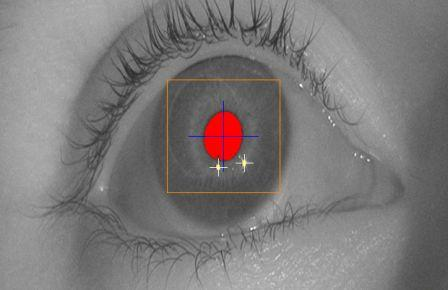
\includegraphics[width=0.5\textwidth, height=30mm]{figures/screenGazeTracker.jpg}
\vspace{-3mm}
\end{center}
\caption{\textbf{The Open Source ITU Gaze Tracker tracking one eye.} The
features tracked in the image are the pupil center and two corneal reflections.}
\label{screenGazeTracker}
\end{figure}


\subsection{Experimental Setup}
The goal of the tests was to compare how well the users could dictate test using the gaze method correction when comparing with the voice and mouse and keyboard correction methods. For this purpose, a graphical user interface (GUI) was designed and implemented in order to run the experiments.

\subsubsection{Participants}
Twenty participants made part of the tests. Among them, there was a random number of native and non-native English speakers (male and female) once that the speech recognition system performs differently with non-native English speakers.

\subsubsection{Apparatus}
The experiment counted with a GUI programmed in Python 2.6 using the Qt 4.8.4 Framework, by Digia, and the PyQt 4.9.6 bindings. The speech recognition system incorporated in the interface was provided by the Microsoft Speech Application Programming Interface (SAPI), with the version 5.1 of the SDK, in the Windows 7 operational system. In order to track the gaze, a Tobii Gaze Tracker was used together with the Tobii SDK 3.0 RC1 for Windows.

\subsubsection{Experimental task}
Each participant had to try and dictate 10 sentences in less than one minute using each correction modality, a total of 30 sentences. The sentences and the correction modality were randomly selected in order to avoid biased measurements.

For this goal, the user interface, presented in \ref{guiExampleEdited} showed the correction modality, the target sentence and the number of the trial, varying from 1 to 30, on the top of the screen. When a sentence was understood by the speech recognizer, the words were presented on the center of the screen. These words could be corrected in three different ways, determined by the correction modality:
\begin{itemize}
  \item Mouse and keyboard: On clicking a word with the mouse, a pop-up menu would be shown with similar words, which could be selected also by clicking. When the desired word was not presented as an alternative, clicking again on the word would generate a line edit and allow to type the desired word;
  \item Voice: A pop-up menu could be generated by saying the command "correct" followed by the desired word to correct. In this mode, the alternatives words are preceded by a number that, when pronounced, selects the related word. When the desired correction was not presented in the pop-up menu, pronouncing again the word would refresh the menu with a new list of alternatives.
  \item Gaze: Looking to a word for 2 seconds would generate the pop-up menu with alternatives. Similarly, the alternative word could be selected by fixing the gaze for 2 seconds. Pronouncing again the word would refresh the menu with new alternatives.
\end{itemize}

On the bottom of the screen, three options buttons were available when a word was being corrected, i.e., with the pop-up menu opened: "Close correction", which would close the pop-up menu of alternatives, "Remove", that would delete the word, and "Delete sentence", which would delete all the previously pronounced words. Also, a "Next" button, when possible, allowed the user to proceed to the next sentence. These buttons could be activated either by using the mouse or the correction modality.

When the user had correctly pronounced the desired sentence, the "Next" button and the target sentence would become green to indicate that the user could go to the next trial. However, if the desired sentence was not reached in less than 60 seconds, the "Next" button and the target sentence would become red, indicating that the user has failed to correct the sentence in suitable time and could start the next trial.

\begin{figure}[ht]
\begin{center}
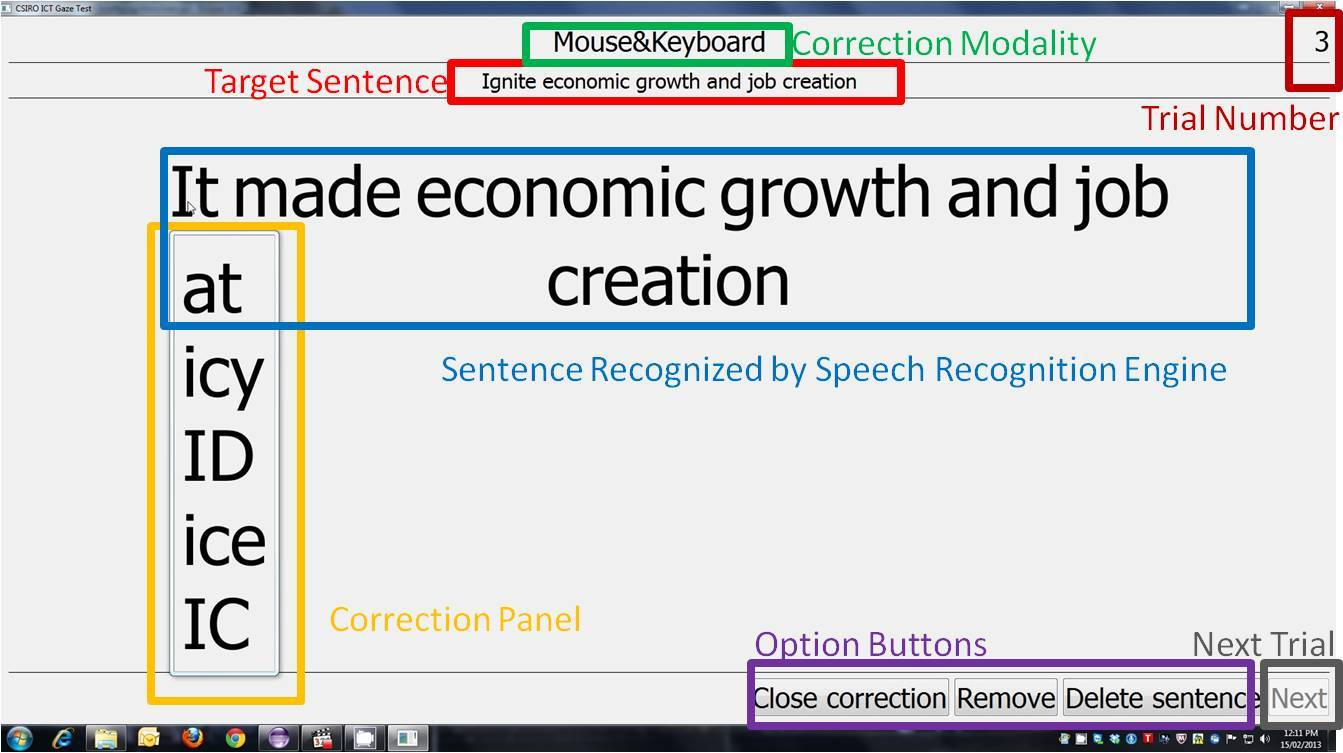
\includegraphics[width=0.75\textwidth]{figures/guiExampleEdited.jpg}
\vspace{-3mm}
\end{center}
\caption{\textbf{GUI used in the experiments.}}
\label{guiExampleEdited}
\end{figure}


\subsubsection{Measures}
During the experiment, time was measured, which would stop if the sentence was successfully pronounced or if the user failed and clicked on the "Next" button.

When correcting by mouse and keyboard, the mouse displacement and keystrokes were recorded.

Each sentence also had a recording indicating whether the trial has failed or not.

Lastly, both the pronounced and the target sentence were recorded, later used to calculate the Damerau�Levenshtein distance between them. This distance revels how far two strings are considering four basic operations: insertion, deletion, and substitution of a single character, and transposition of two adjacent characters. (http://dl.acm.org/citation.cfm?id=363994)



\section{Results}
More plain text.

\section{Discussion}
Bla bla

\section{Conclusion}
Bli bli bli

\bibliographystyle{plain}
\bibliography{library}

\end{document}
